\documentclass[border=4pt]{standalone}
\usepackage[T1]{fontenc}\usepackage{helvet}\renewcommand{\familydefault}{\sfdefault}
\usepackage[helvet]{sfmath}
\usepackage{tikz}\usepackage{pgfplots}\pgfplotsset{compat=1.16}
\begin{document}
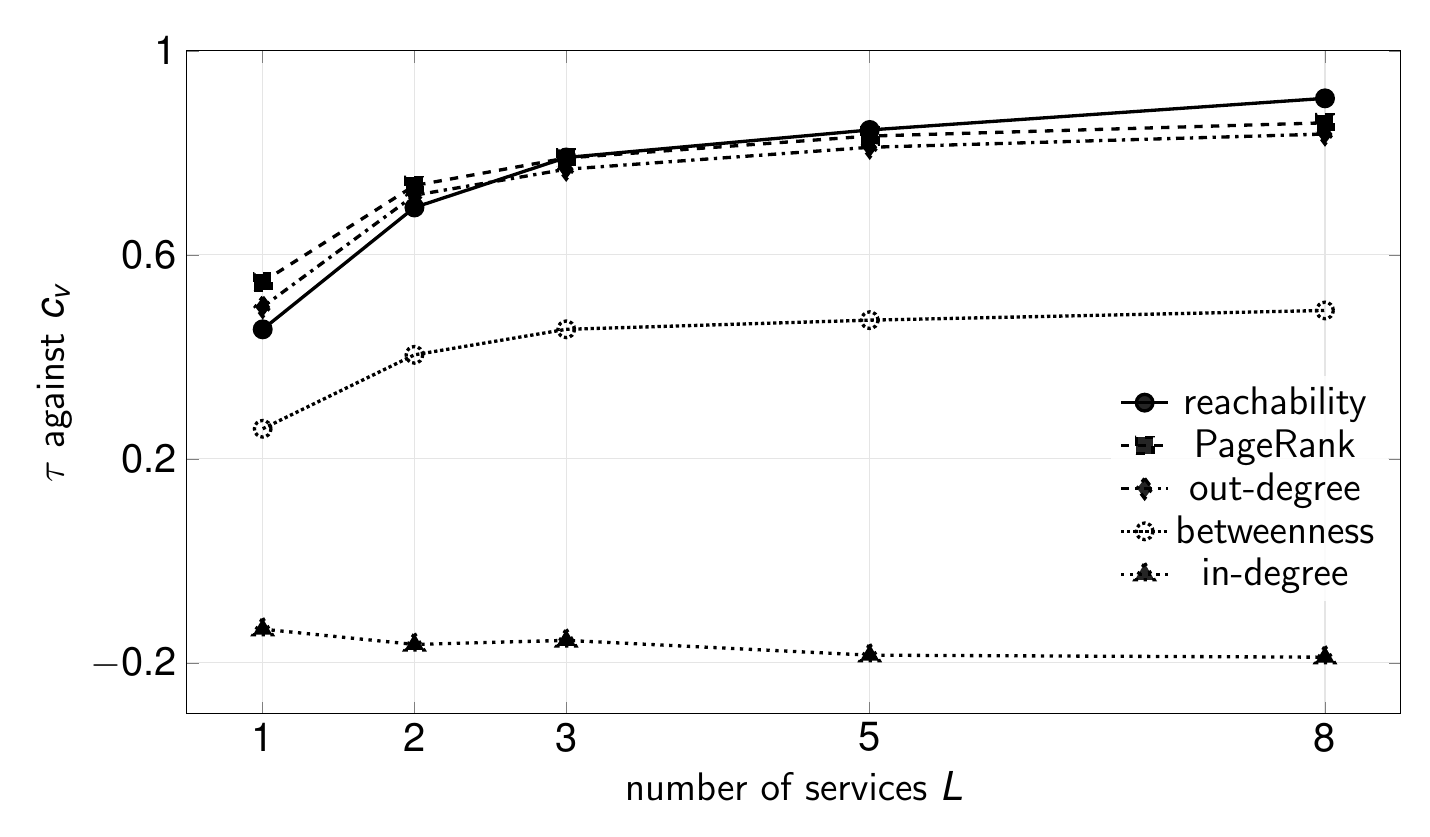
\begin{tikzpicture}
\begin{axis}[
  width=17cm, height=10cm,
  xlabel={number of services $L$}, ylabel={$\tau$ against $c_v$},
  xmin=0.5, xmax=8.5, ymin=-0.3, ymax=1.0,
  xtick={1,2,3,5,8}, ytick={-0.2,0.2,0.6,1.0},
  tick label style={font=\Large}, label style={font=\Large},
  grid=major, grid style={gray!20},
  legend style={font=\Large, at={(0.99,0.34)}, anchor=east, draw=none,
                fill=white, fill opacity=0.85, text opacity=1}]
\addplot[very thick,mark=*,mark size=3pt,black] coordinates
  {(1,0.454)(2,0.693)(3,0.791)(5,0.845)(8,0.907)};
\addlegendentry{reachability}
\addplot[very thick,mark=square*,mark size=3pt,black,dashed] coordinates
  {(1,0.547)(2,0.736)(3,0.790)(5,0.833)(8,0.859)};
\addlegendentry{PageRank}
\addplot[very thick,mark=diamond*,mark size=3.6pt,black,dashdotted] coordinates
  {(1,0.498)(2,0.717)(3,0.768)(5,0.811)(8,0.837)};
\addlegendentry{out-degree}
\addplot[very thick,mark=o,mark size=3pt,black,densely dotted] coordinates
  {(1,0.259)(2,0.404)(3,0.454)(5,0.472)(8,0.491)};
\addlegendentry{betweenness}
\addplot[very thick,mark=triangle*,mark size=4pt,black,dotted] coordinates
  {(1,-0.134)(2,-0.164)(3,-0.156)(5,-0.185)(8,-0.189)};
\addlegendentry{in-degree}
\end{axis}
\end{tikzpicture}
\end{document}
